\classheader{11-20-2017}

\section*{Computing a Fundamental Group}

We've only thought about the fundamental group in abstract.  Does there even exist a space with nontrivial fundamental group? (Obviously the answer is yes...)

Let's look at $\R$ as a covering space of $\S^1$.\\

	\begin{figure}[!htb]
	\centering
	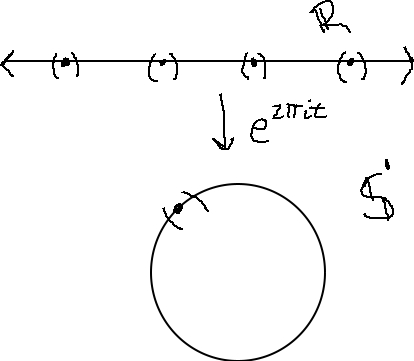
\includegraphics[scale=.5]{images/rs1covsp}
	\caption{A covering space $\R\rightarrow\S^1$}
	\label{fig:r_s1_cov}
\end{figure}

In a covering space, the number of sheets at any point is always the same, which is not necessarily true of a local homeomorphism.

\definition{If $\pi:\tilde{M}\rightarrow M$ is a covering space and $p\in M$ is a point, then a neighborhood $U$ of $p$ is \textbf{evenly covered} if any component of $\pi^{-1}(U)$ is homeomorphic to $U$ via $\pi$.}

\definition{The preimage of $p$ is called the \textbf{fiber} above $p$.}

\example{Recall our construction of the torus using $\R^2/\Z^2$.  This is a covering space $\pi(x,y)\mapsto (e^{2\pi i x},e^{2\pi iy}).$
	
		\begin{figure}[!htb]
		\centering
		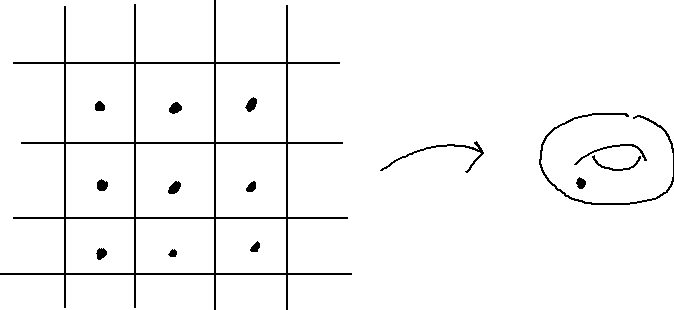
\includegraphics[scale=.5]{images/r2totorcov}
		\caption{A covering space $\R^2\rightarrow \mathbb{T}$}
		\label{fig:r2tor_cov}
	\end{figure}


We've also seen before the two-to-one covering of the annulus to the M\"obius strip

	\begin{figure}[!htb]
	\centering
	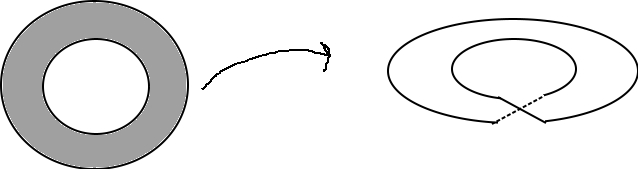
\includegraphics[scale=.5]{images/anntomob}
	\caption{The two-to-one covering of the M\"obius strip}
	\label{fig:annmob_cov}
\end{figure}


We can observe that if $\pi:\tilde{M}\rightarrow M$ is a covering space and $\gamma$ is a path in $\tilde{M}$, then $\pi\circ\gamma$ is a path in $M$.

\begin{theorem}[Path Lifting Property]
	If $\pi:\tilde{M}\rightarrow M$ is a covering space, $\gamma$ a path in $M$, and $\ast$ a point in $\tilde{M}$ in $\pi^{-1}(\gamma(0))$, then there exists a unique path $\tilde{\gamma}$ in $\tilde{M}$ such that $\gamma=\pi\circ\tilde{\gamma}$ such that $\tilde{\gamma}(0)=\ast$.
\end{theorem}
\begin{proof}
	The idea is to take a finite open cover of the path, choose a sheet, and look at the inverse images of the cover on that sheet, then construct the path in those sets.
	
	Each point $p\in\gamma(I)$ has an evenly covered neighborhood $U_p$, so $\{U_p\}$ is an open cover of $\gamma(I)$.  Since $I$ is compact, we can pick a finite subcover $\{U_i\}_{i\in\N}$.  Arrange each of these in order by their infimum along the interval.  The cover $\{\gamma^{-1}(U_i)\}$ of $I$ has some Lebesgue number $\delta$.  Thus any interval $[x-\frac{\delta}{4},x+\frac{\delta}{4}]$ is entirely inside of some $\gamma^{-1}(U_i)$.
	
	Now we have a collection of intervals $I_j=[(j-1)\frac{\delta}{4},j\frac{\delta}{4}]$ for $j=1,2,\dots,\lceil\frac{\delta}{4}\rceil$ and $I=[0,1]=I_1\cup I_2,\dots\cup (I_{\lceil\frac{\delta}{4}\rceil}\cap [0,1])$.  As $\gamma(I_j)$ is entirely inside some evenly covered set, as long as $\gamma((j-1)\frac{\delta}{4})$ has a lift, all of $\gamma(I_j)$ does.  Doing this for all subintervals, we can build a lift of $\gamma(I)$ to some path in $\tilde{M}$ $\tilde{\gamma}$.
\end{proof}

We can observe that if $\pi:\tilde{M}\rightarrow M$ is a covering space and $\gamma$ is a path in $\tilde{M}$, then $\pi\circ\gamma$ is a path in $M$.
\begin{theorem}
	This composition gives rise to an injection of fundamental groups, $\pi_*:\pi_1(\tilde{M},\tilde{x})\rightarrow \pi_1(M,\pi(\tilde{x})$.
\end{theorem}
